\begin{figure}[htb!]
\centering
\begin{tabular}{c}
%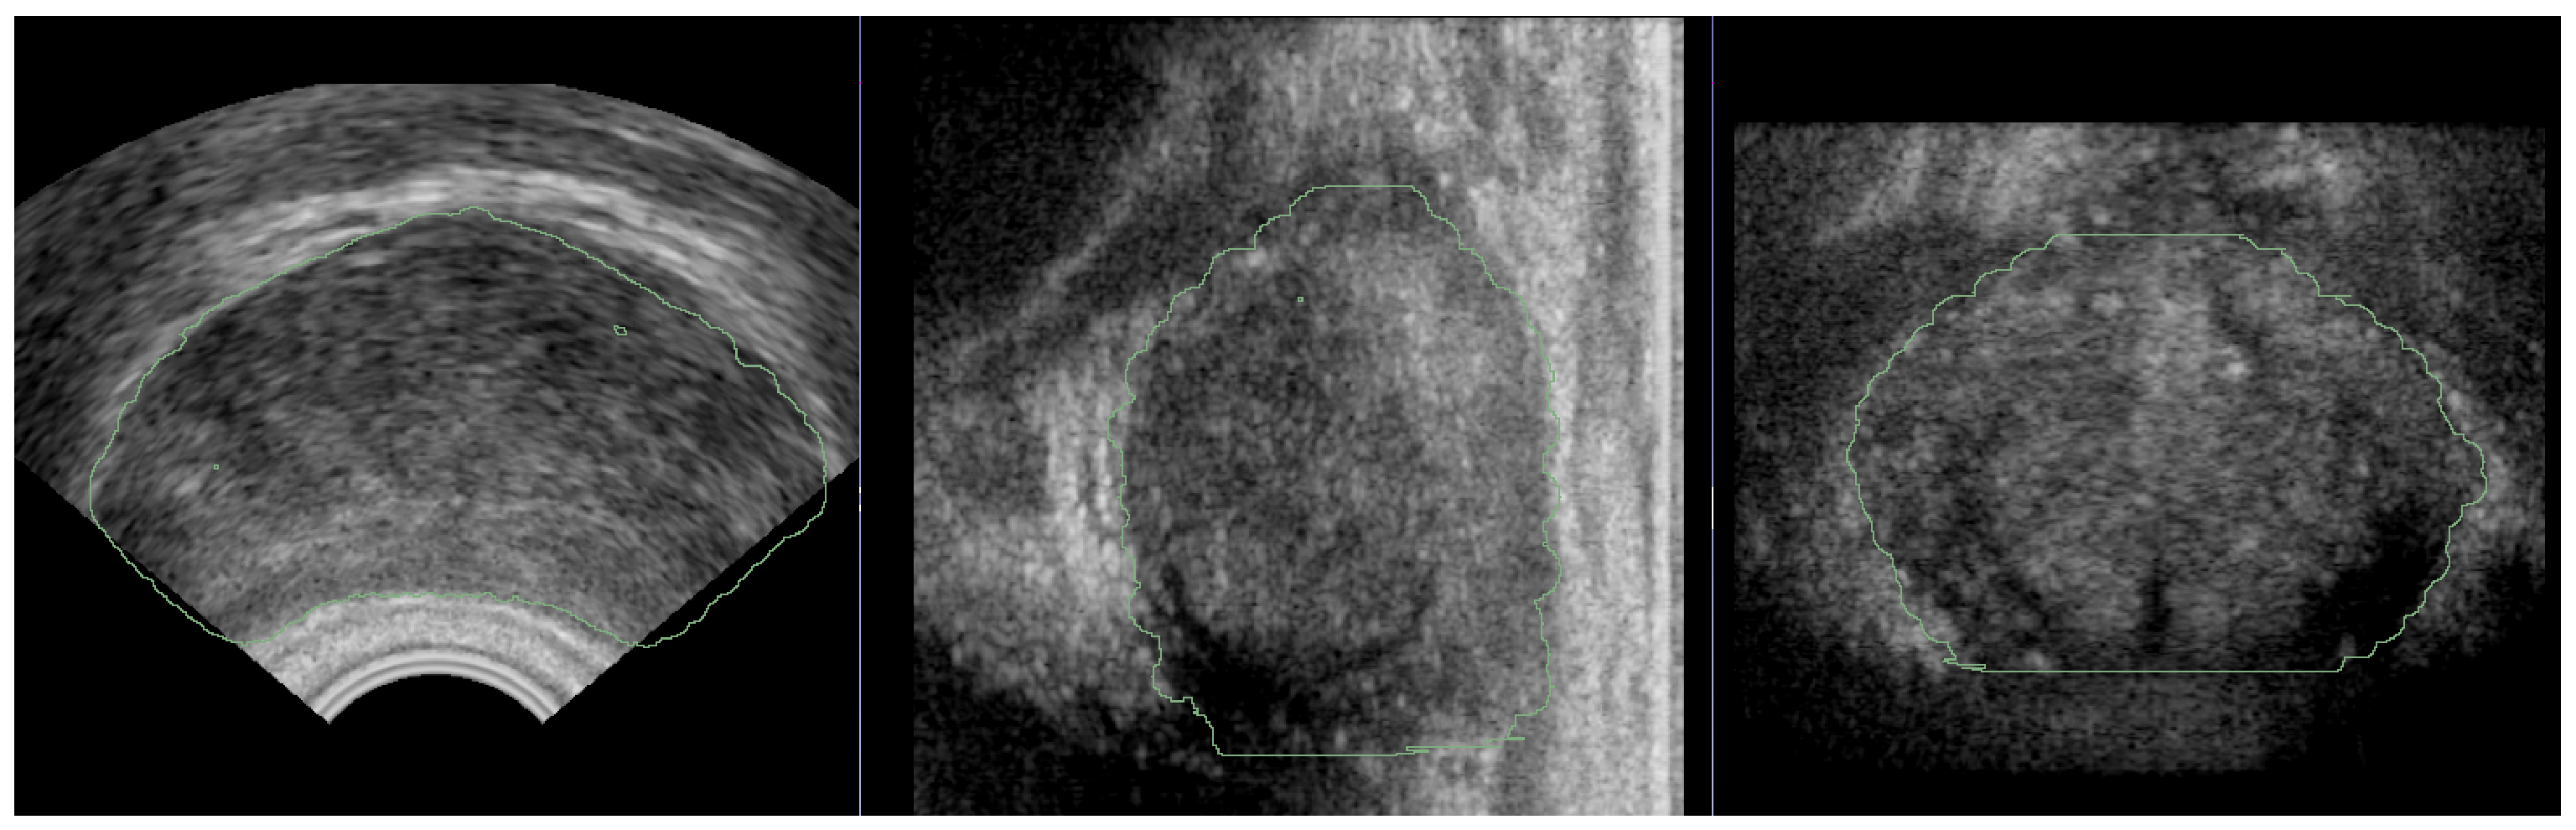
\includegraphics[width=1.0\textwidth]{figs/Bmode_CapsuleSegs.eps} \\
%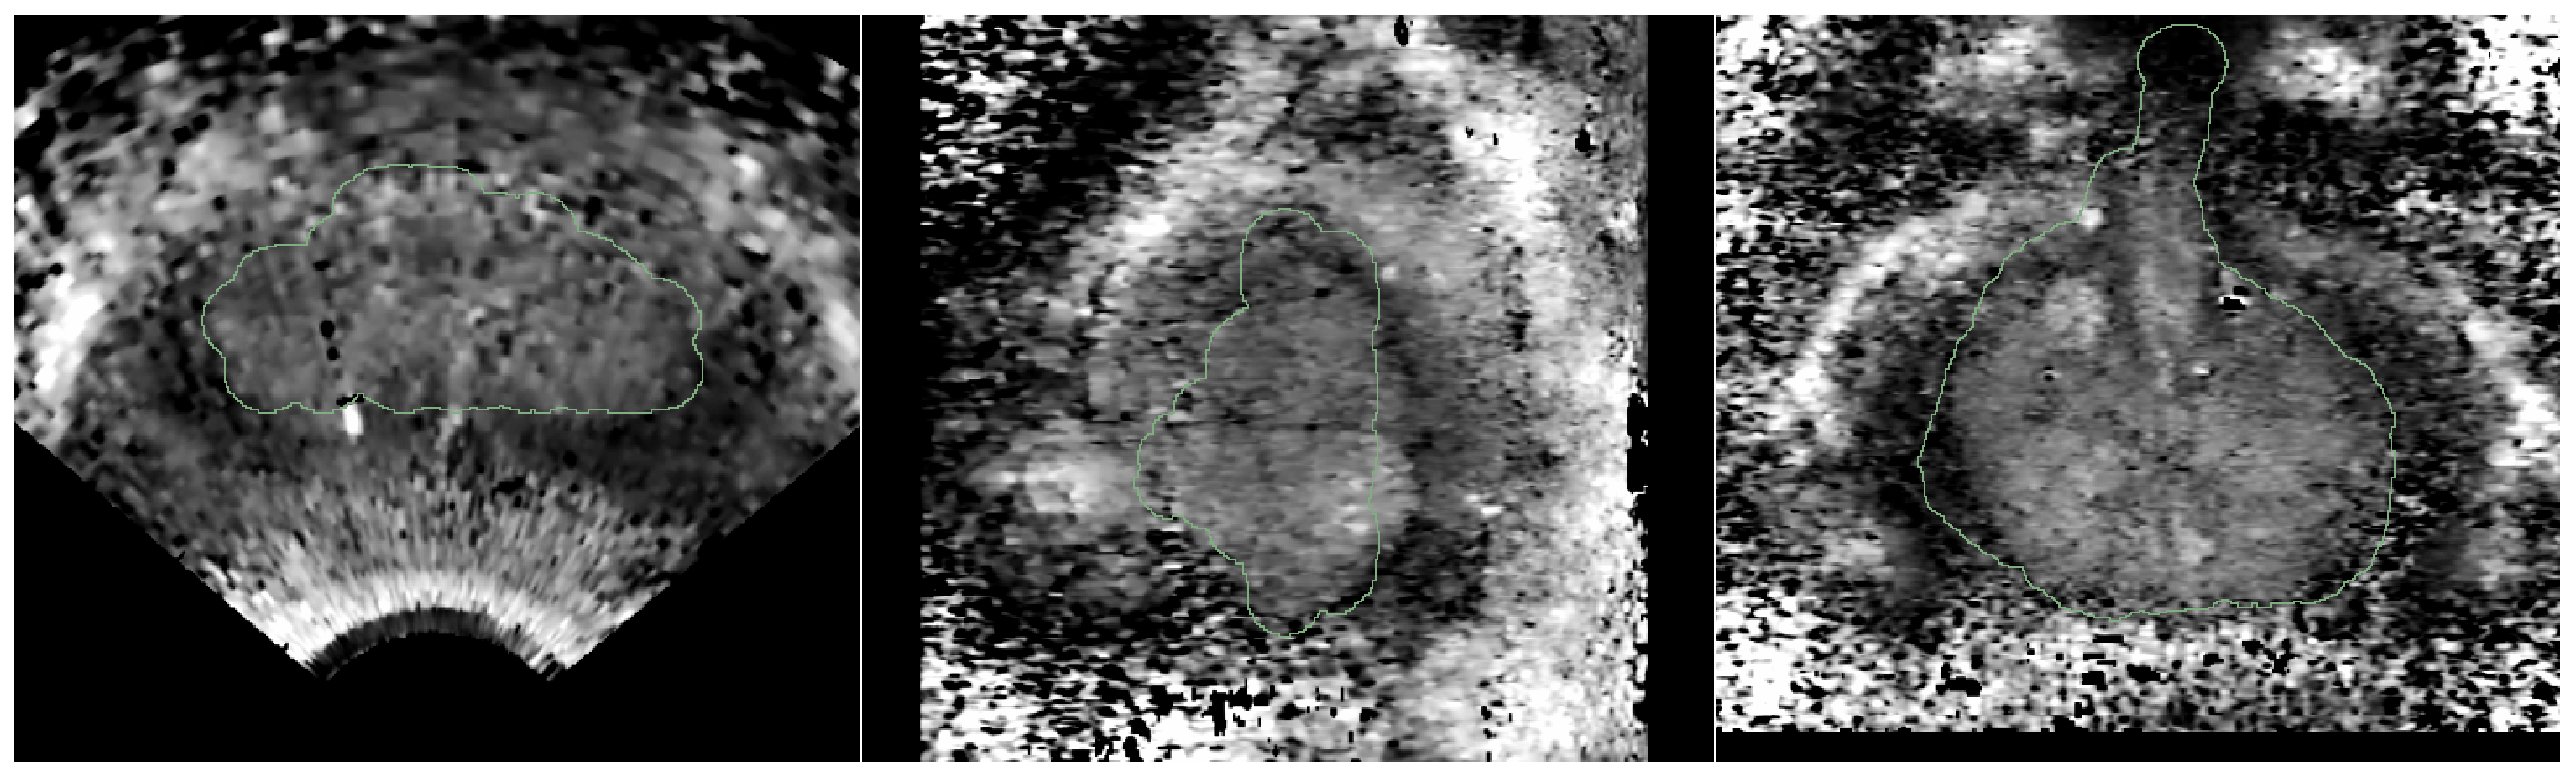
\includegraphics[width=1.0\textwidth]{figs/ARFI_CGsegs.eps} \\
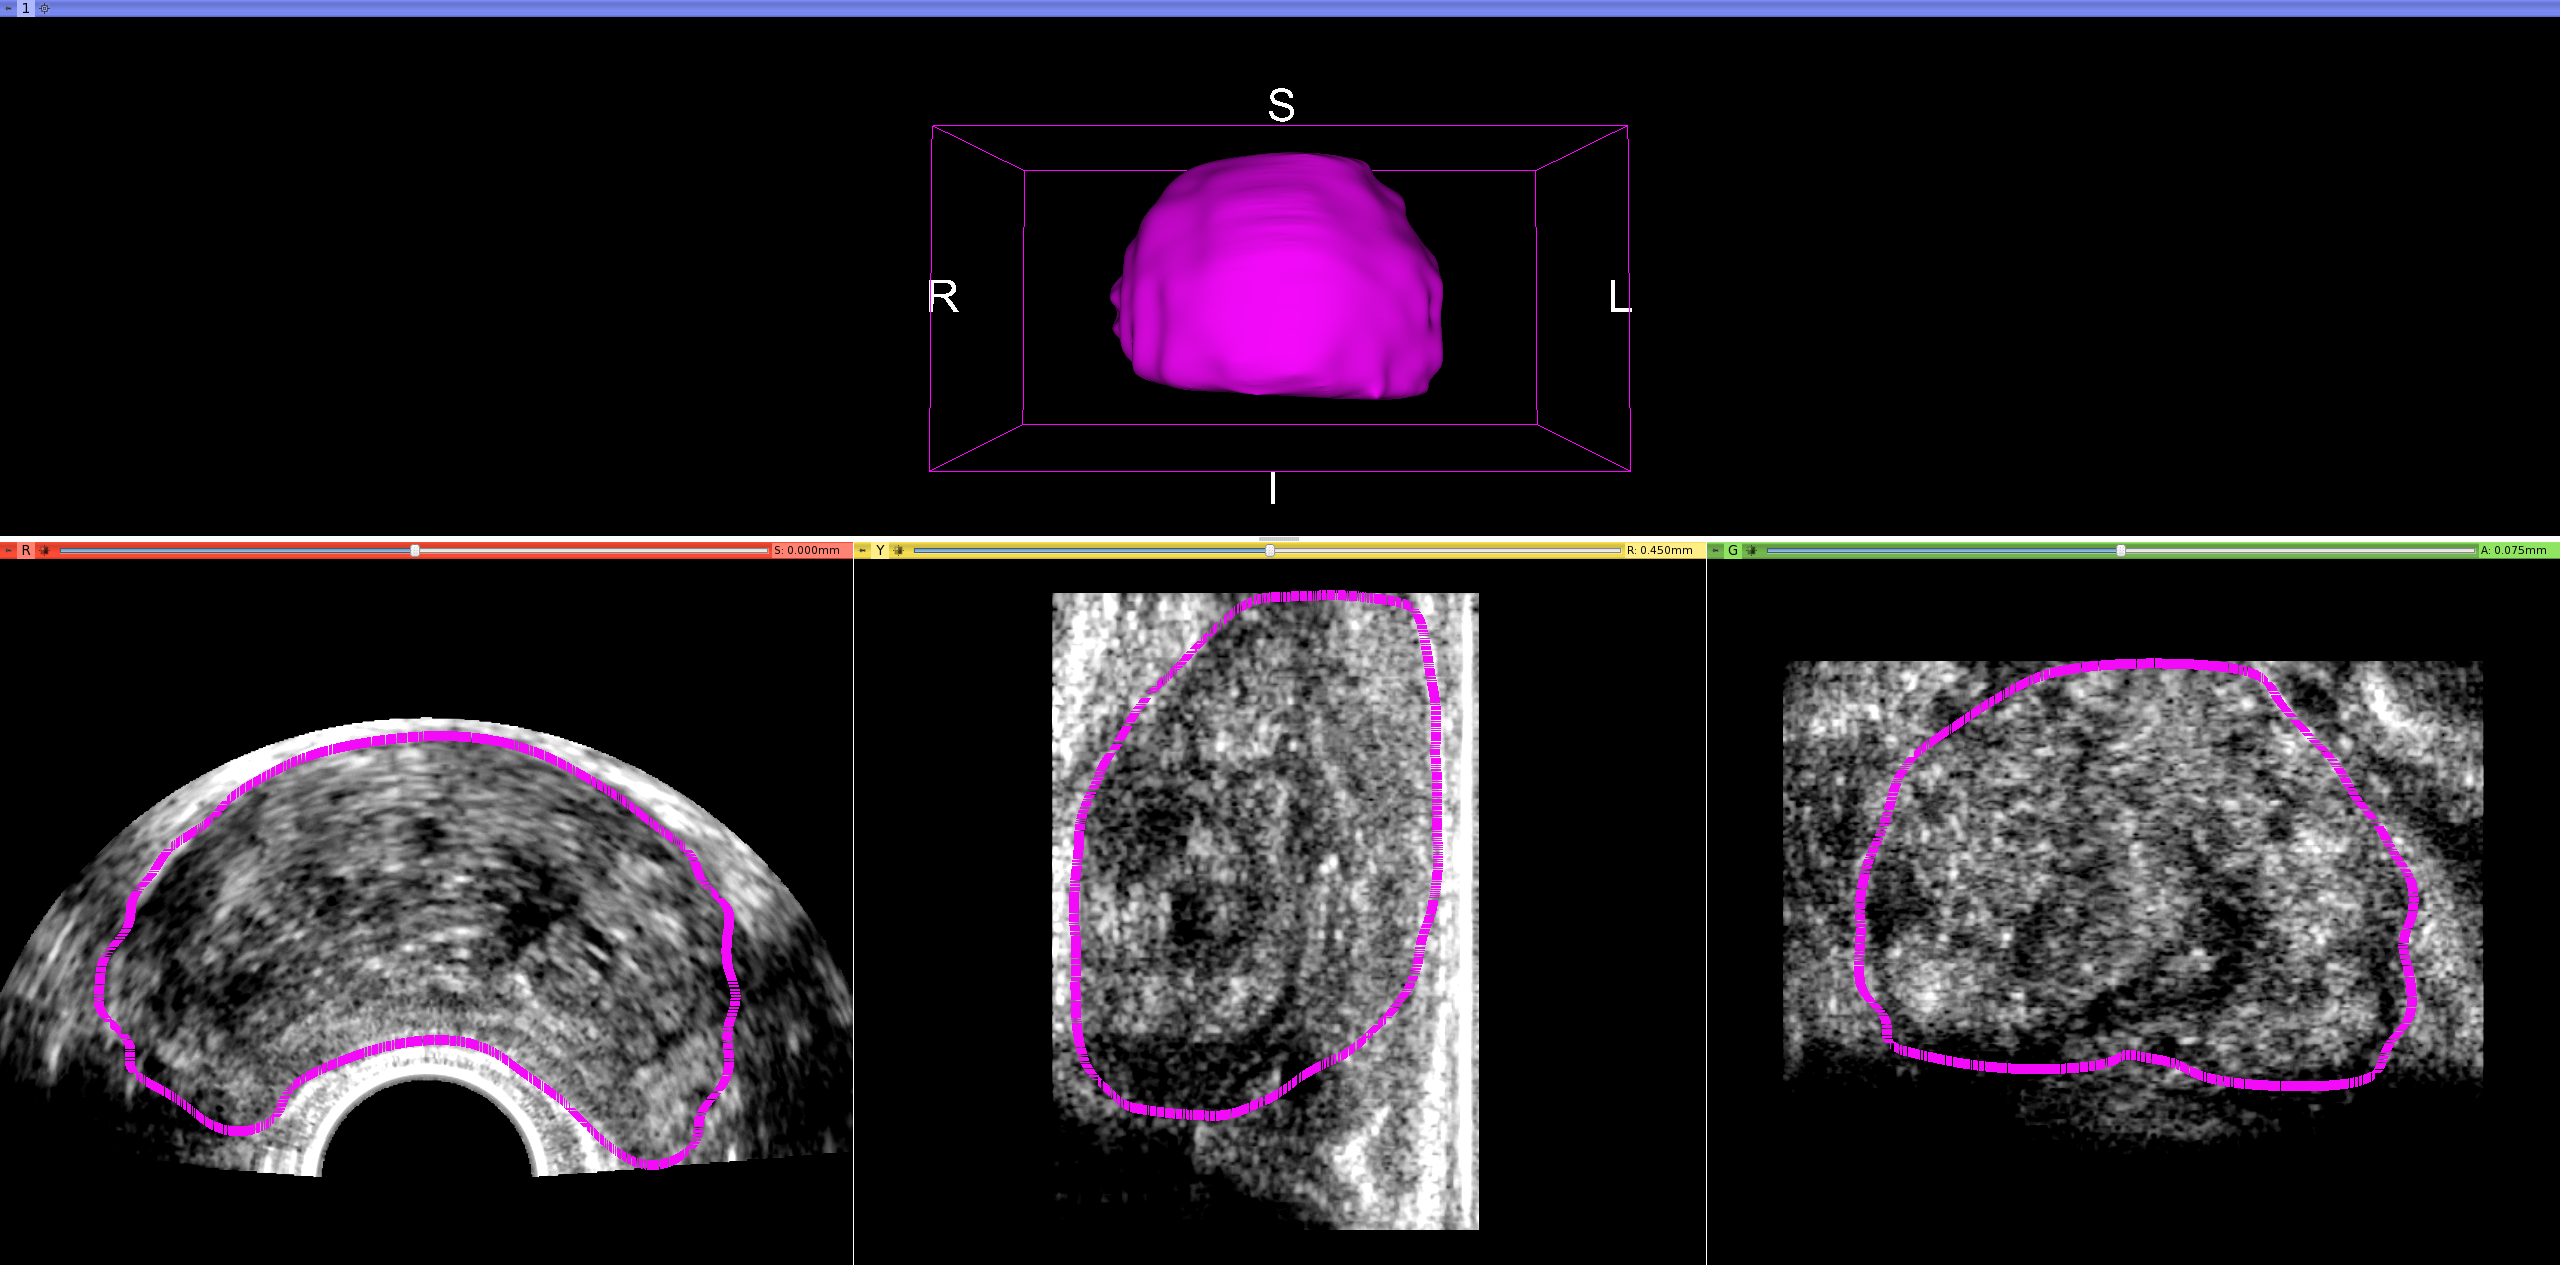
\includegraphics[width=0.8\textwidth]{zach/us_capsule_seg_model.png} \\
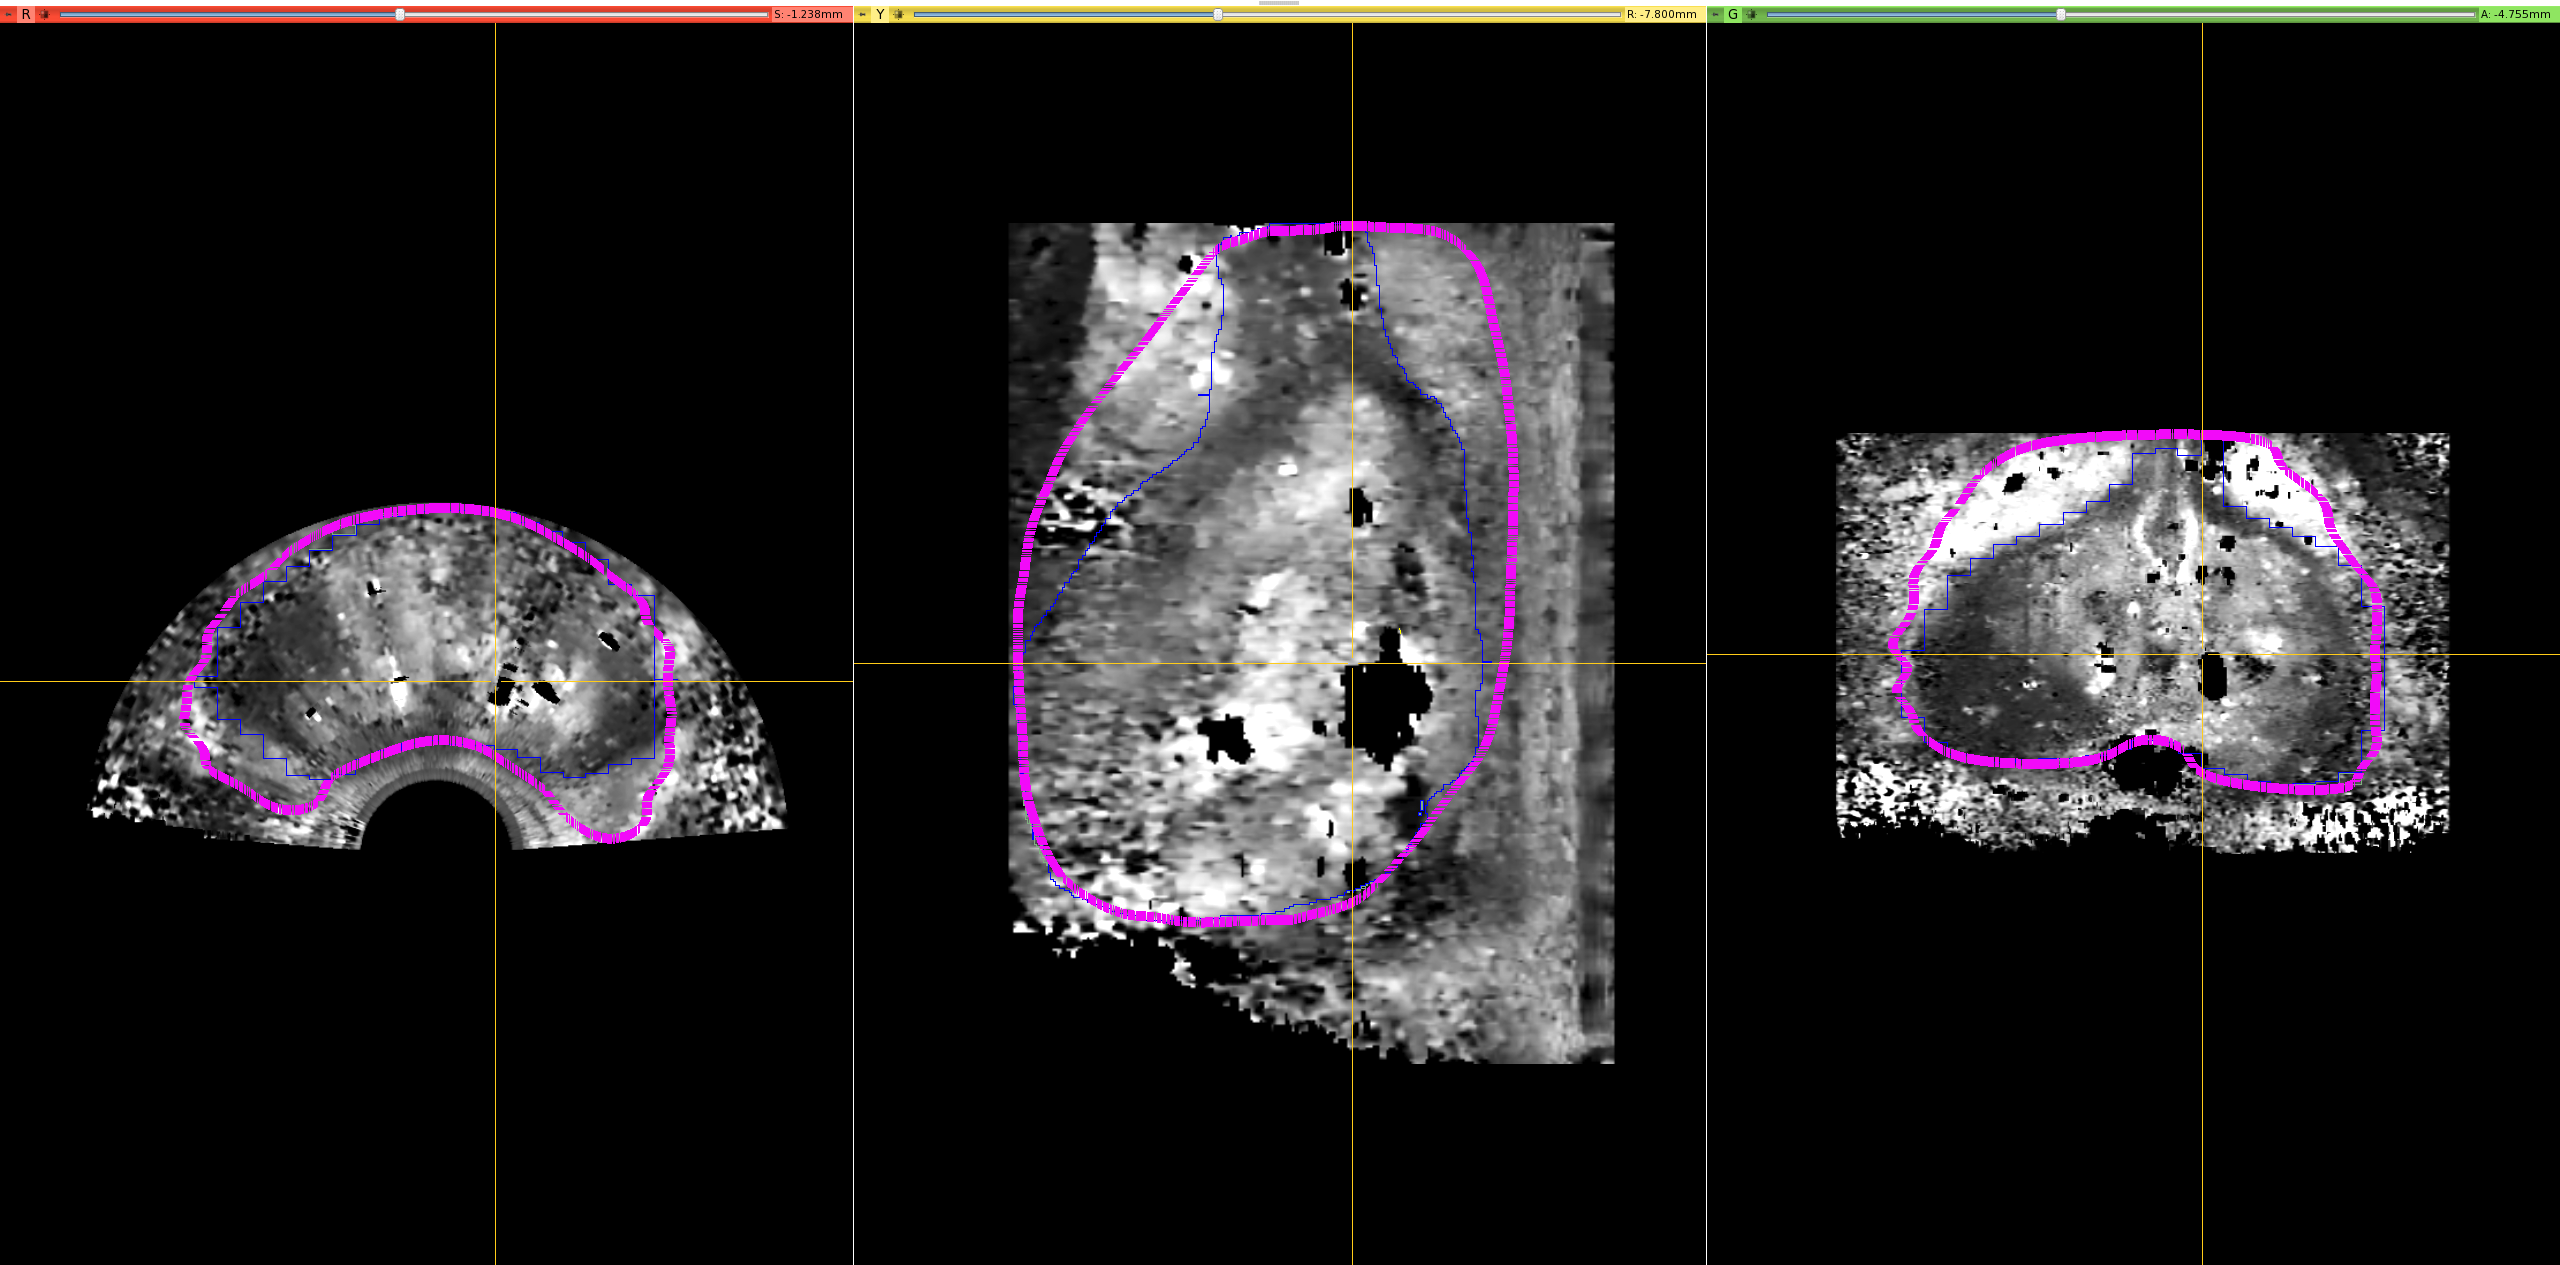
\includegraphics[width=0.8\textwidth]{zach/arfi_central_seg.png} \\
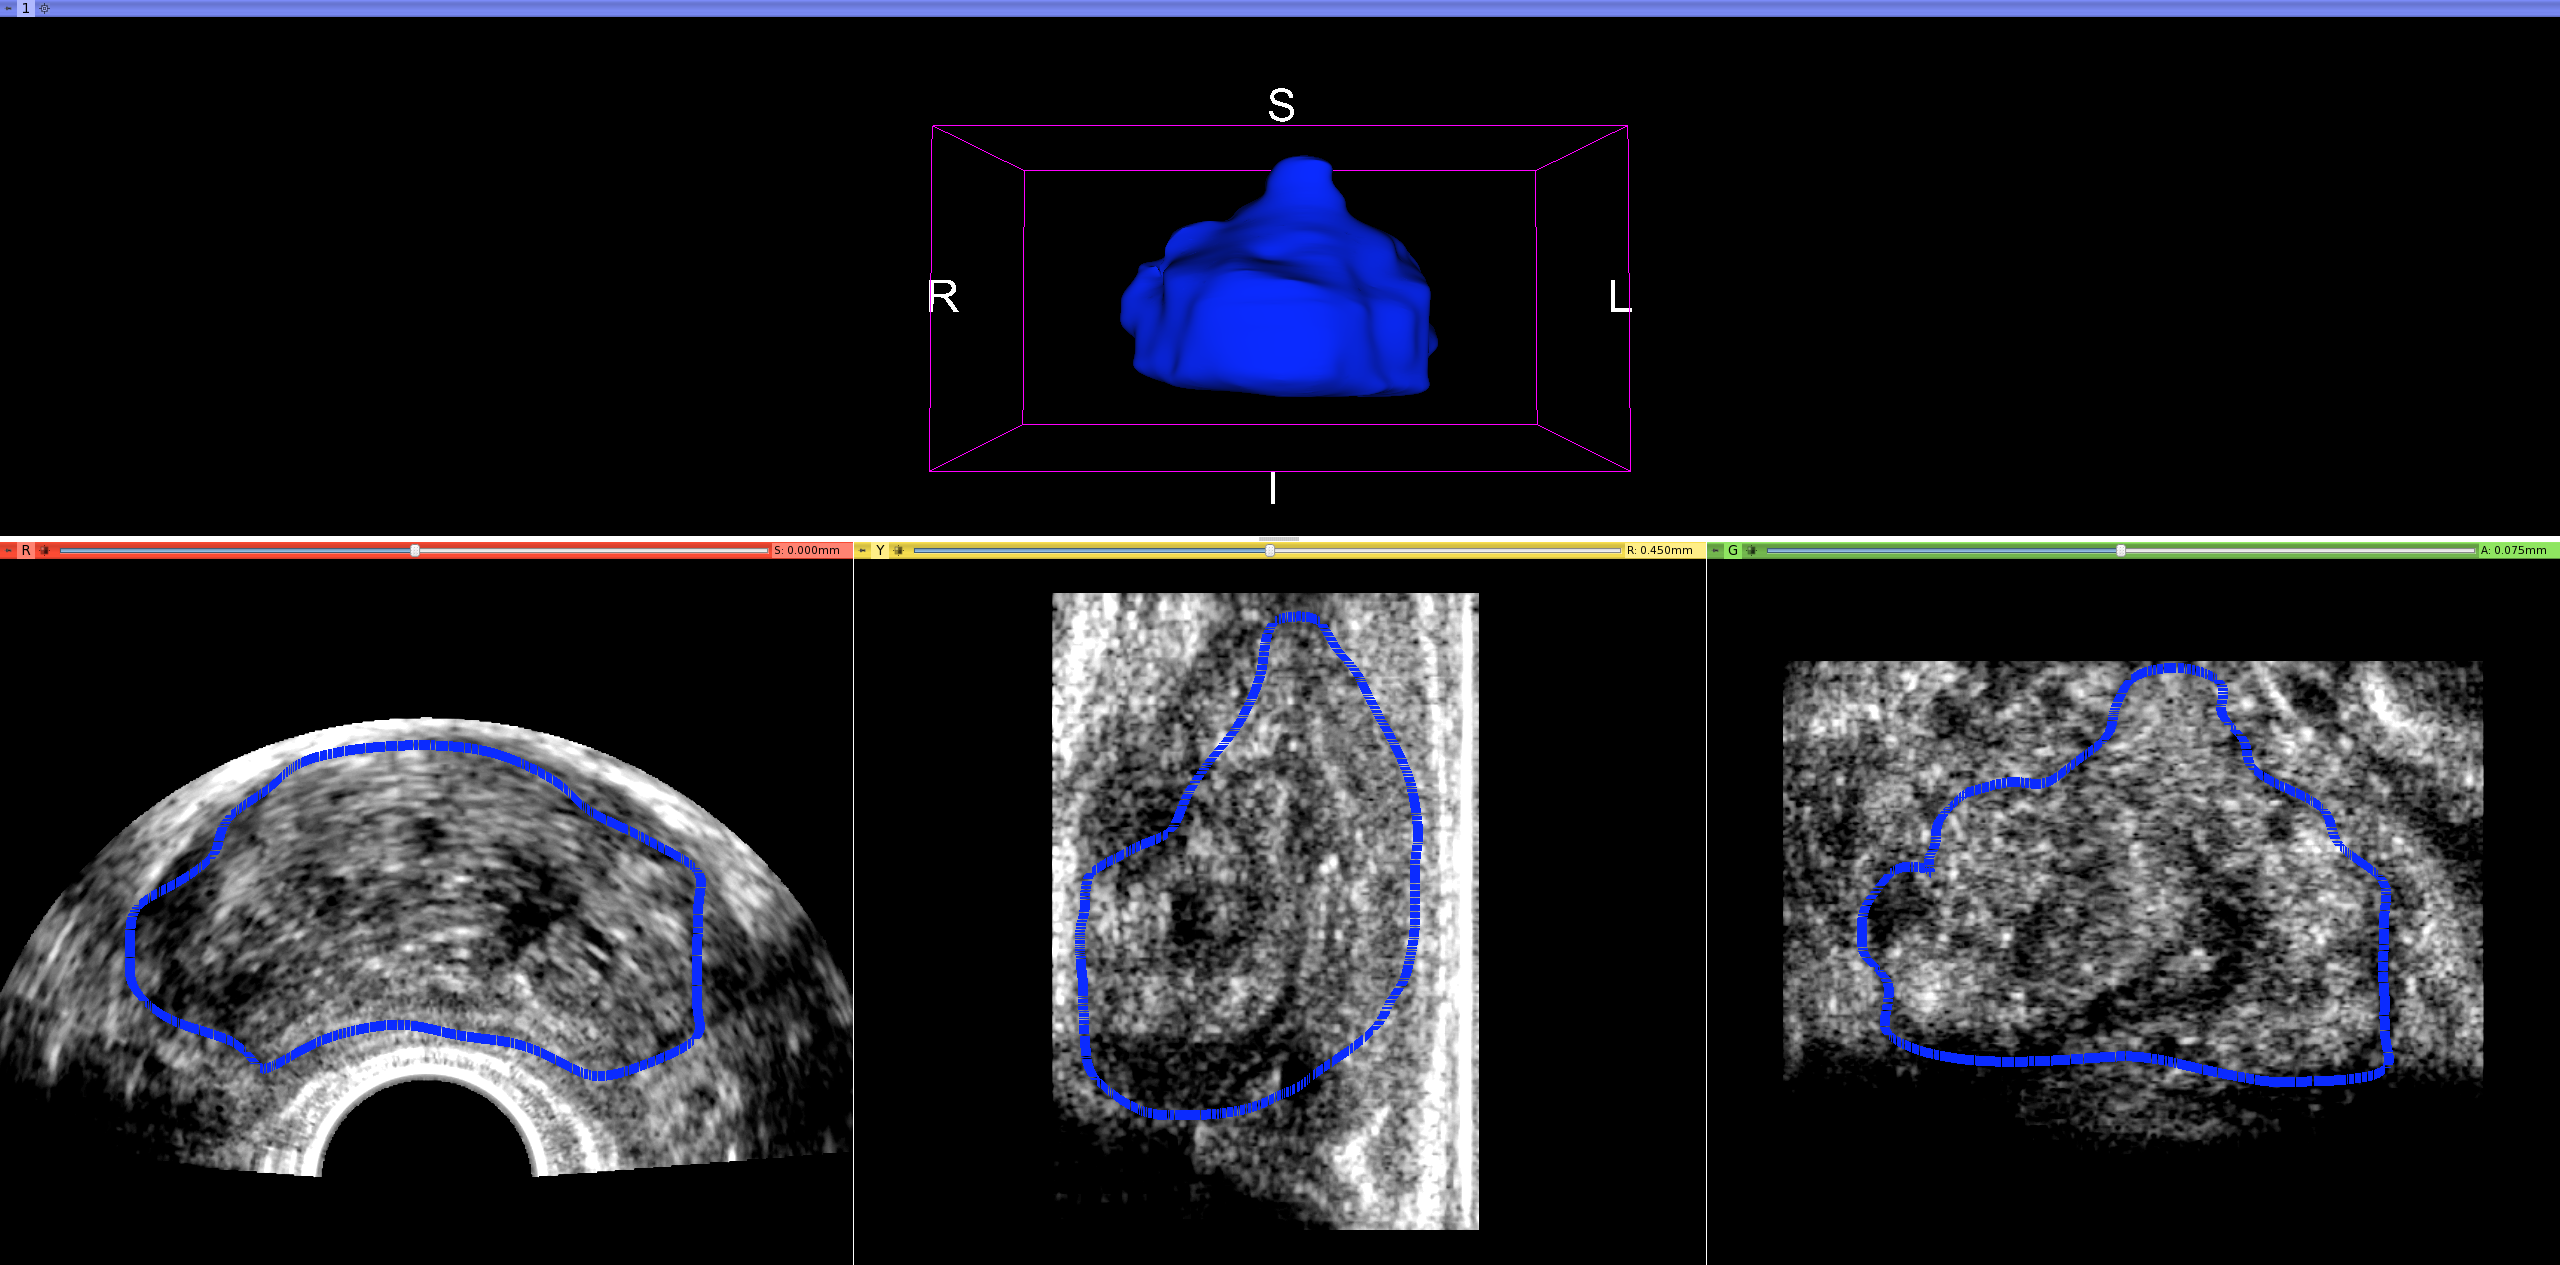
\includegraphics[width=0.8\textwidth]{zach/us_central_seg_model.png} \\
\end{tabular}
\caption{TOP ROW: B-mode capsule segmentation using all three orthogonal
    planes.  The primary segmentation plane is sagittal (second pane), however
    the axial (first pane) and coronal (third pane) are used to guide this
    segmentation because as the label map is built up, the intersections of
    the label map in the axial and sagittal planes can be viewed as well. The
    block-like character of the axial/coronal sections of the label map are a
    direct result of downsampling.  MIDDLE ROW: ARFI central gland segmentation
    (blue) with the capsule model (pink) overlaid for guidance during
    segmentation.  BOTTOM ROW: Demonstrates the modeled capsule with slice
    intersections on the axial, sagittal, and coronal planes respectively (all
    pink). This model was built up from the label map created in the B-mode
    capsule segmentation.}
\label{fig:arfi_segs} 
\end{figure}
